% @Author: Mouna REKIK
% @Date:   2024-10-11 / 12:30
%%%%%%%%%%%%%%%%%%%%%%%%%%%%%%%%%%%%%%%%%%%%%%%%%%%%%%%%%%%%%%%%%%%%%%%%%%%%%%

\chapter{Étude conceptuelle}
\begin{spacing}{1.2}
\minitoc
\thispagestyle{MyStyle}
\end{spacing}
\newpage

\section{Introduction}
L’objectif de ce chapitre est de présenter les fondements conceptuels et technologiques qui ont guidé la conception de notre plateforme. Nous introduisons d’abord Nous introduisons d’abord les exigences et l’architecture globale basée sur les microservices, puis les services cloud associés, avant de détailler l’évolution vers une approche multi-agents. Enfin, nous comparons les principaux frameworks RAG et modèles de langage utilisés, afin de justifier les choix retenus.

\section{Spécification des exigences}
Avant de plonger dans les détails architecturaux, il est essentiel de définir les principaux acteurs ainsi que les exigences qui ont guidé la conception de la plateforme.
\subsection{Identification des acteurs}
Pour mieux illustrer les interactions entre les acteurs principaux et le système, la figure suivante présente un diagramme de cas d’utilisation global. On distingue deux types d’acteurs :\\
- l’Administrateur: responsable de la création et de la configuration des chatbots (chargement de documents, personnalisation d’actions, rédaction de questions-réponses)\\
- l’Utilisateur final: qui utilise le chatbot pour initier une conversation et discuter.
\begin{figure}[H]%
    \centering
    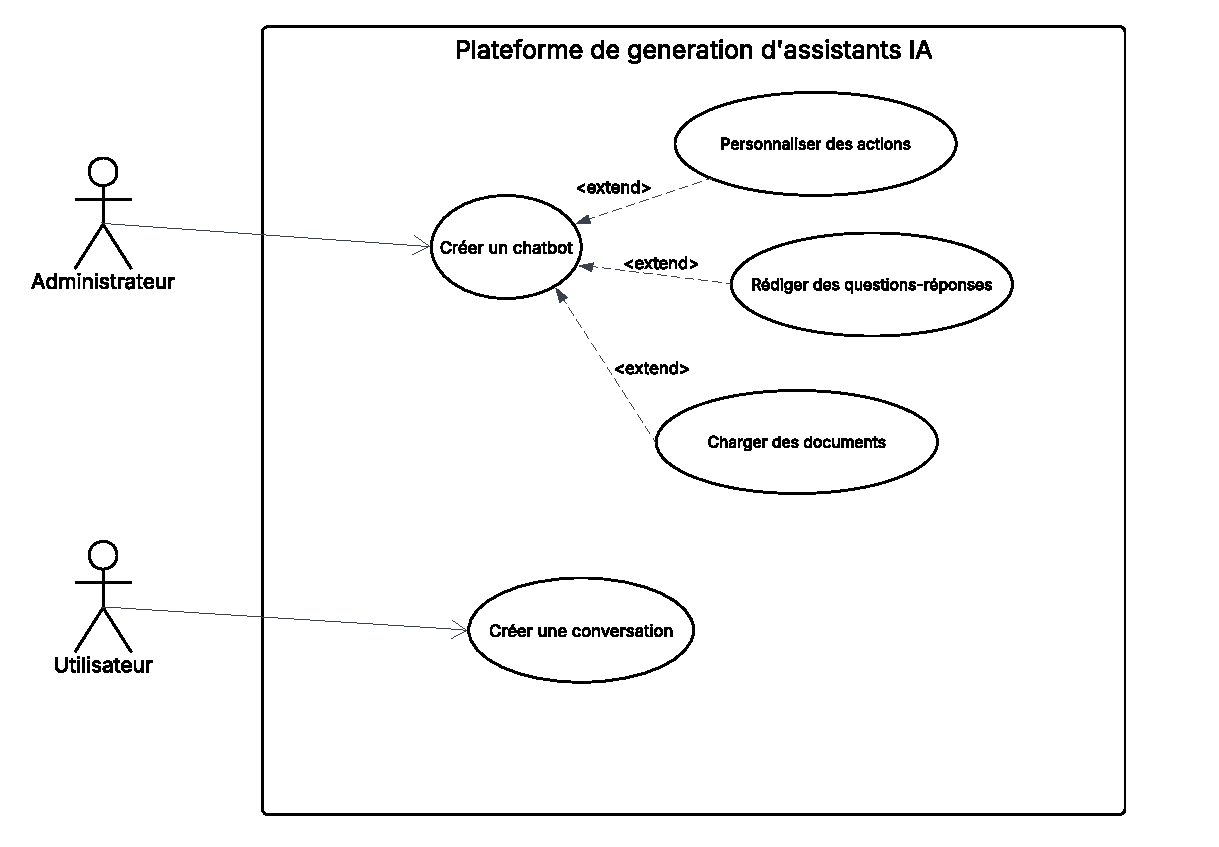
\includegraphics[keepaspectratio,height=8cm]
    {images/diag_uc.pdf}%
    \caption{Diagramme de cas d'utilisation global}%
\end{figure}

\subsection{Exigences fonctionnelles}
Les exigences fonctionnelles définissent les capacités principales que la plateforme doit offrir pour répondre aux besoins des utilisateurs. Elles incluent :
\begin{itemize}[label=\textbullet]
\item Création, modification et suppression de chatbots : Les administrateurs doivent pouvoir créer de nouveaux chatbots, les modifier selon les besoins et les supprimer si nécessaire.
\item Gestion d’une base de connaissances multi-sources : La plateforme doit supporter l’intégration de documents variés (PDF, CSV, TXT), d’URLs et de paires questions/réponses (Q/R) pour enrichir les connaissances des chatbots.
\item Configuration d’actions personnalisées : Les chatbots doivent pouvoir exécuter des actions spécifiques, telles que des appels à des API externes, l’envoi d’e-mails ou des recherches web.
\item Supervision de plusieurs agents via une interface administrateur : Une interface dédiée permet aux administrateurs de superviser et gérer plusieurs agents simultanément.
\item Intégration frontale : Des widgets et interfaces conversationnelles intuitives doivent permettre aux utilisateurs finaux d’interagir facilement avec les chatbots, y compris via des intégrations multiplateformes comme des bulles de conversation sur des sites web ou des connecteurs vers des applications tierces (ex. : WhatsApp).
\end{itemize}
\subsection{Exigences non fonctionnelles}
Les exigences non fonctionnelles sont définies en suivant les caractéristiques de qualité de la norme ISO/IEC 25010 \cite{iso}. Cependant, en raison des contraintes du projet, certaines exigences sont partiellement satisfaites dans cette phase, avec des plans pour les renforcer dans les itérations futures. Les exigences prioritaires et leur état d’avancement sont décrits ci-dessous :
\begin{itemize}[label=\textbullet]
\item Performance : La plateforme vise un temps de réponse réduit pour l’utilisateur final, avec un objectif de latence inférieur à 2 secondes pour les interactions conversationnelles sous une charge modérée. Actuellement, la latence moyenne est de 3 seconde pour les requêtes simples, mais des optimisations supplémentaires sont nécessaires pour les charges élevées.
\item Compatibilité (interopérabilité) : Les microservices doivent communiquer via des API REST standardisées pour une intégration fluide avec des systèmes externes (ex. : CRM, ERP). Cette exigence est pleinement satisfaite grâce à l’utilisation d’API REST bien documentées, permettant une communication efficace entre les microservices et les services Azure.
\item Utilisabilité : L’interface utilisateur (frontend) doit être intuitive, avec une courbe d’apprentissage minimale. Les widgets sont intégrables en moins de 5 minutes, comme requis. Cependant, des tests utilisateurs supplémentaires sont prévus pour améliorer l’ergonomie de l’interface administrateur.
\item Fiabilité : La plateforme doit garantir des réponses précises, cohérentes et sans hallucinations, avec un objectif maximal de réponses conformes aux paires Q/R et au contexte RAG. Actuellement, la fiabilité des réponses n'est pas 100 \% pour les requêtes complexes, mais des améliorations, notamment via l’architecture multi-agents, sont en cours pour réduire les hallucinations et atteindre l’objectif.
\item Maintenabilité : L’architecture microservices permet l’ajout de fonctionnalités sans perturber les services existants. Cette exigence est pleinement satisfaite grâce à Azure DevOps.
\item Scalabilité : La plateforme doit supporter une augmentation de la charge. Ceci est assuré via un serveur nginx.
\end{itemize}
Ces exigences servent de base pour l’architecture globale et les choix technologiques décrits dans les sections suivantes.
\section{Architecture globale de la plateforme}
La conception de notre application repose sur une architecture microservices déployée sur Microsoft Azure. Cette approche permet de garantir la scalabilité et la maintenabilité du système. Chaque microservice est conçu comme une unité indépendante, avec une responsabilité spécifique, ce qui facilite à la fois l’évolution de l’application et l’intégration de nouvelles fonctionnalités.

La Figure suivante présente une vision englobante de la plateforme. Elle met en évidence les quatre microservices principaux, ainsi que les services cloud associés (Azure OpenAI Service, Azure Blob Storage, Azure SQL Server, etc.), qui constituent l’infrastructure technique supportant notre solution.
\begin{figure}[H]%
    \centering
    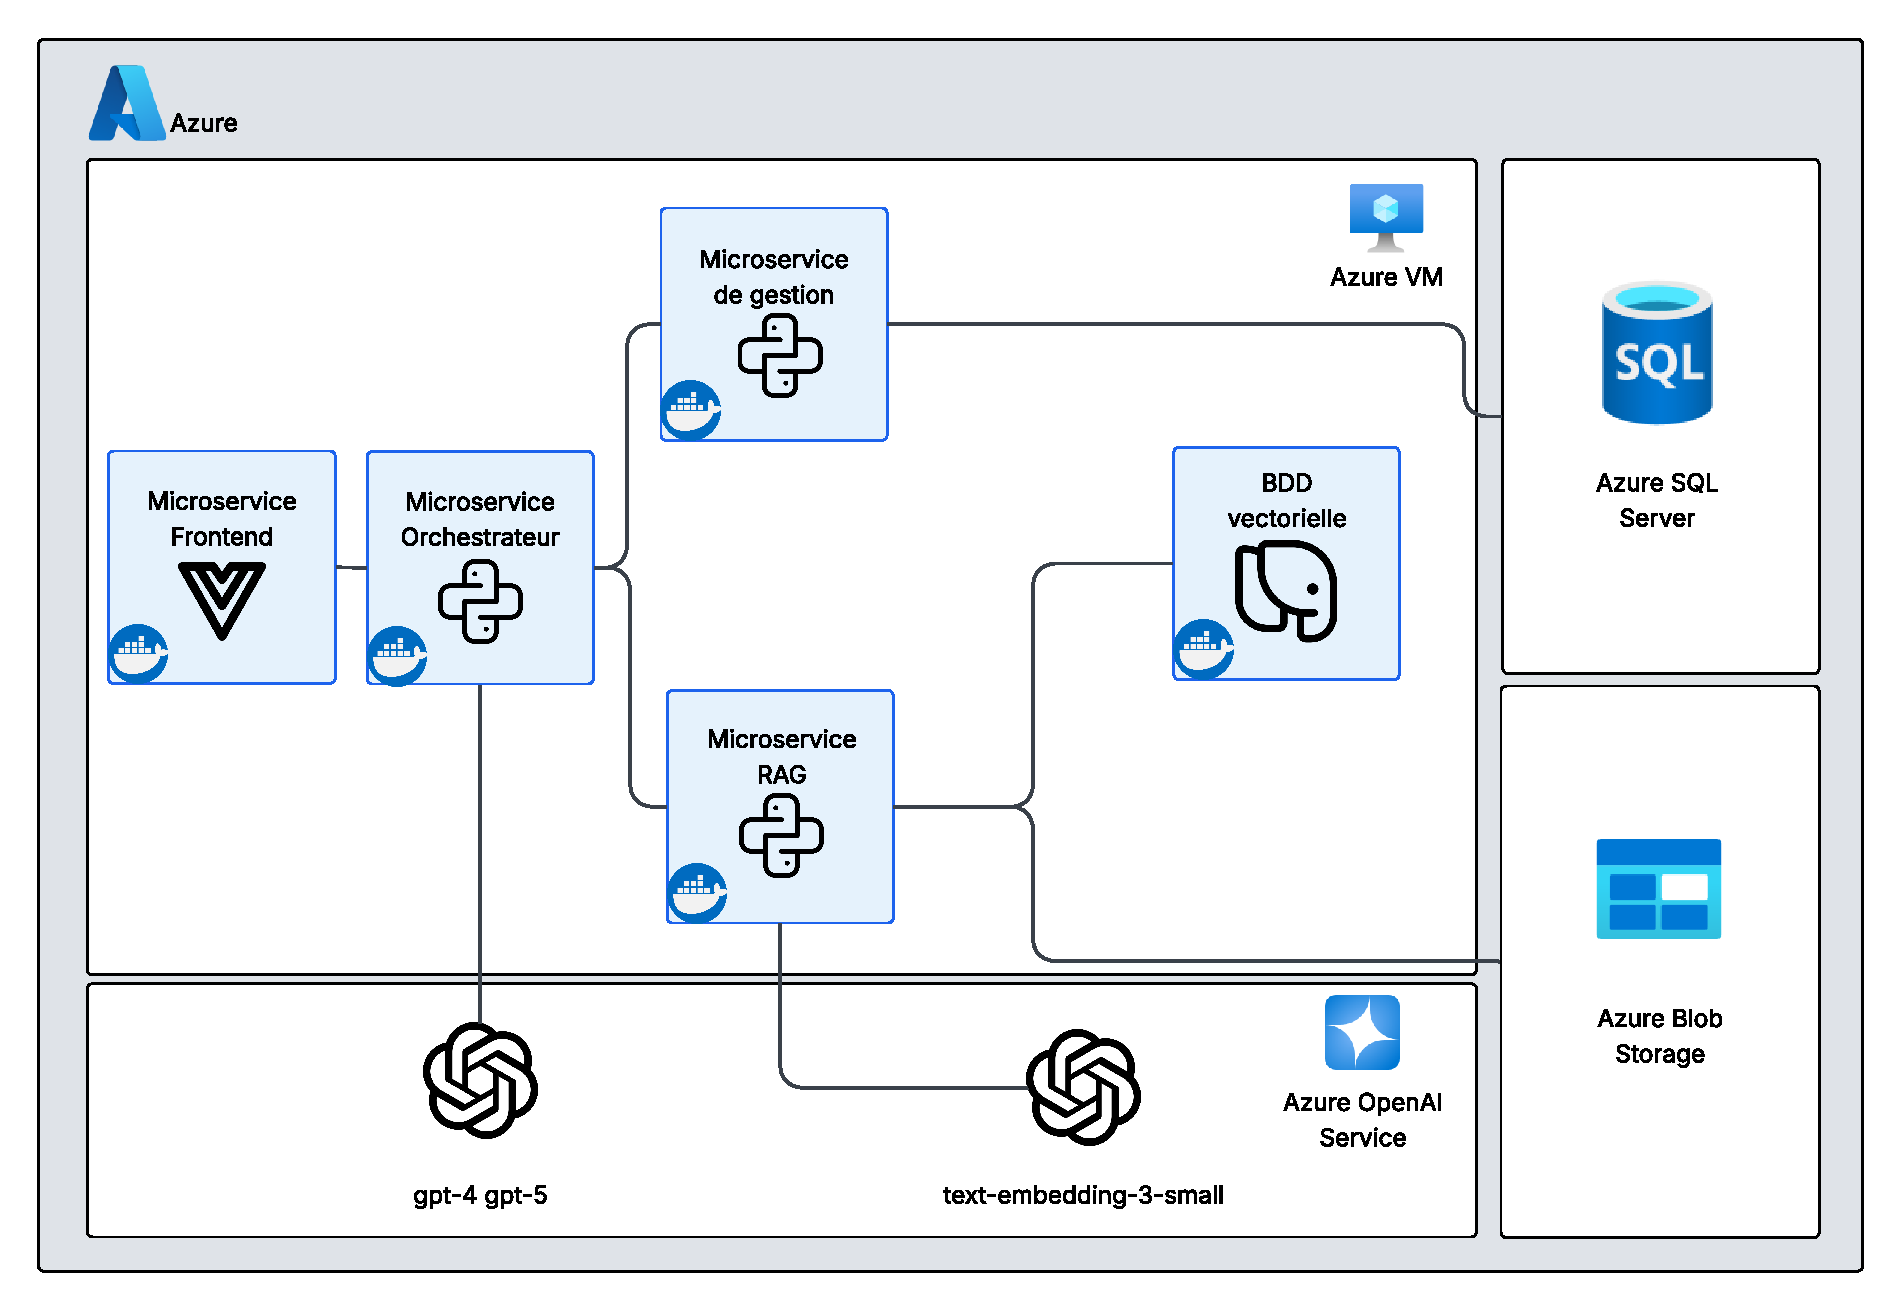
\includegraphics[keepaspectratio,height=8cm]
    {images/arch_glob.pdf}%
    \caption{Architecture globale}%
\end{figure}

Le premier composant clé de l’architecture est le microservice frontend, développé avec Vue.js, qui constitue le point d’entrée principal pour les utilisateurs. Ce microservice gère l’interface, permettant aux administrateurs de configurer les chatbots et aux utilisateurs finaux d’interagir avec les assistants personnalisée via une interface conversationnelle moderne. En s’appuyant sur des widgets, tels qu’une bulle de conversation intégrable sur des sites web ou des connecteurs vers des applications tierces comme WhatsApp, le frontend garantit une accessibilité multiplateforme, alignée avec l’objectif d’offrir une expérience utilisateur fluide et adaptable à divers contextes professionnels.

Au cœur de l’architecture, le microservice orchestrateur joue un rôle central en coordonnant les interactions entre les différents composants du système. Il reçoit les requêtes du frontend, les analyse, et les redirige vers les microservices appropriés en fonction des besoins, assurant ainsi une communication fluide et cohérente. Cette coordination est essentielle pour garantir que les actions personnalisées, telles que les appels API ou les recherches web, soient exécutées de manière efficace, en adéquation avec les besoins spécifiques des utilisateurs finaux. L’orchestrateur s’appuie sur Azure AI Foundry pour la gestion LLMs.

Le microservice de gestion centralise les opérations internes, notamment la configuration des chatbots, la gestion des paramètres, et les opérations CRUD (création, lecture, mise à jour, suppression). Ce composant permet aux administrateurs de définir les informations des assistants virtuels, telles que leur nom, leur domaine d’application, ou leurs permissions, tout en garantissant une isolation modulaire pour une scalabilité optimale. En s’intégrant avec Azure SQL Database, ce microservice stocke et gère les données relationnelles, telles que les configurations des chatbots, tandis que l’utilisation d’Azure Blob Storage permet de gérer les fichiers associés, comme les bases de connaissances importées sous forme de PDF, CSV ou TXT.

Pour illustrer les relations entre les entités, la figure suivante présente un diagramme de classes, détaillant les classes clés (chatbots, actions, conversations) et leurs interactions, offrant une vision technique de l’architecture.
\begin{figure}[H]%
\centering
\includegraphics[keepaspectratio,height=8cm]
{images/copy_diag_cls.pdf}
\caption{Diagramme de classes}%
\end{figure}

Enfin, le microservice RAG est dédié au traitement des fichiers importés en combinant une base de connaissances vectorisée avec des modèles d’embedding. Ce microservice indexe les documents importés et effectue des recherches sémantiques pour fournir des réponses pertinentes et contextualisées. En s’appuyant sur Azure OpenAI Service pour la génération de réponses, garantissant une précision et une personnalisation conformes aux attentes des utilisateurs.

\section{Services cloud associés}
Notre application repose sur plusieurs services gérés par la plateforme Microsoft Azure, qui offrent des garanties en termes de performance, sécurité et scalabilité. Ces services soutiennent l'architecture microservices en fournissant l'infrastructure nécessaire pour le stockage, le traitement des données et l'intégration des modèles IA, contribuant directement à l'objectif global de la plateforme : permettre une gestion flexible et personnalisée des chatbots. Chaque service est intégré de manière spécifique aux microservices, assurant une coordination fluide et une adaptabilité aux besoins des administrateurs et des utilisateurs finaux.
\subsection{Azure OpenAI Service}
Azure OpenAI Service \cite{azure-openai-docs} fournit un accès sécurisé à des LLMs avancés, tels que GPT-4, GPT-4o-mini et GPT-5 pour la génération de contenu, ainsi que des modèles d'embedding comme text-embedding-3 pour la vectorisation des données. Ce service agit comme le cœur des capacités conversationnelles de la plateforme, en permettant au microservice RAG de réaliser des recherches sémantiques et de générer des réponses contextuelles basées sur les bases de connaissances importées. Par exemple, lors de l'indexation de documents ou de la réponse à des requêtes utilisateurs, le microservice RAG invoque ces modèles via des requêtes HTTP vers les endpoints mis en marche, garantissant une intégration native avec l'écosystème Azure. Cette approche renforce la personnalisation des chatbots en offrant des interactions précises et actualisées, tout en maintenant la confidentialité des données.

\subsection{Azure Blob Storage}
Azure Blob Storage \cite{azure-blob-docs} offre une solution scalable pour le stockage d'objets non structurés, tels que des documents PDF, des fichiers CSV ou des images, qui servent de base à la construction des connaissances des chatbots. Ce service est étroitement lié au microservice de gestion, qui gère le chargement et la configuration des fichiers utilisateurs, ainsi qu'au microservice RAG pour l'indexation efficace des données lors des interactions conversationnelles. Grâce à son intégration avec les SDK Python utilisés dans les microservices, Azure Blob Storage facilite le traitement de volumes importants de données sans limitations majeures, supportant ainsi de multiples formats de fichiers. Cette capacité assure une flexibilité essentielle pour adapter les assistants virtuels aux besoins spécifiques des utilisateurs en optimisant les coûts et la performance globale de l'architecture.
\subsection{Azure SQL Database}
Azure SQL Database \cite{azure-sql-docs} gère les données relationnelles de la plateforme, incluant les historiques de conversations, les configurations des chatbots et les paramètres d'accès. Ce service est principalement exploité par le microservice de gestion pour les opérations CRUD et par l'orchestrateur pour maintenir la cohérence des échanges entre les composants. Avec ses fonctionnalités de haute disponibilité et d'intégration avec les outils analytiques Azure, il garantit une persistance fiable des données pour isoler les assistants virtuels.
\subsection{Azure AI Foundry}
Azure AI Foundry \cite{azure-ai-foundry} sert comme plateforme centralisée pour la personnalisation, le test et la gouvernance des solutions IA, intégrant des outils pour le suivi des expériences et le déploiement de modèles. Ce service englobe l'ensemble de l'architecture en facilitant la collaboration sur les modèles utilisés par le microservice RAG et l'orchestrateur, permettant par exemple la création d'agents des flux conversationnels complexes. Grâce à son portail unifié et ses SDK, il supporte le développement collaboratif et traçable, aligné sur l'approche agentique de la plateforme. Cette intégration assure une évolution continue des chatbots, en incorporant des outils d'IA variés selon les domaines d'activité, et renforce l'objectif global.

\subsection{Azure DevOps}
Azure DevOps \cite{azure-devops-docs} fournit une plateforme pour la gestion du cycle de vie logiciel, incluant l'hébergement de dépôts de code, l'automatisation des pipelines CI/CD et la collaboration entre équipes. Ce service soutient le déploiement et la maintenance des microservices, tels que le frontend et le backend, en assurant une intégration fluide et une livraison continue des mises à jour. Par exemple, il automatise les tests et les déploiements vers Azure, tout en s'appuyant sur Azure Boards \cite{azure-boards-docs} pour une gestion agile des tâches et des sprints, ce qui facilite la planification et le suivi d'avancement.

\section{Architecture agentique et évolution vers multi-agents}
Avant d’explorer l’évolution vers une architecture agentique, il est essentiel de comprendre le fonctionnement basique de la plateforme, qui constitue la fondation technique sur laquelle repose cette transition (du mono vers multi-agents).
\begin{figure}[H]%
    \centering
    \includegraphics[keepaspectratio,height=8cm]
    {images/fonctionnement_basique.pdf}%
    \caption{Fonctionnement basique}%
\end{figure}
Le processus débute lorsqu’une requête est initiée via le microservice Frontend, qui la transmet au microservice Orchestrateur, chargé de coordonner l’ensemble des opérations. L’Orchestrateur sollicite ensuite le microservice de gestion pour récupérer les paires question/réponse, l’historique des conversations et les actions configurables, stockées dans Azure SQL Server (précisément dans la colonne \texttt{params} et la colonne \texttt{assistant\_info} de la table chatbot). Parallèlement, il interroge le microservice RAG, qui extrait le contexte pertinent de la base de données vectorielle hébergée. Pour traiter ces données, l’Orchestrateur fait appel à Azure OpenAI Service, exploitant les modèles de génération (GPT-4, GPT-5 ...) et d’embedding (text-embedding-3-small) afin d’analyser la requête et générer une réponse adaptée. Cette réponse est ensuite renvoyée au microservice Frontend, complétant ainsi le cycle d’interaction. Cette architecture modulaire pose les bases d’une évolutivité future, notamment avec l’intégration d’approches agentiques plus sophistiquées.

Cette adoption, intégrée au microservice Orchestrateur, a été motivée par les limites rencontrées avec une architecture monolithique basée sur un unique agent ReAct. Progressivement, nous avons évolué vers une orchestration multi-agents, permettant une meilleure robustesse et une réduction remarquable des hallucinations. Cette transition s’appuie sur une infrastructure initiale bien définie, décrite ci-après, qui optimise la coordination entre les microservices et les services cloud pour répondre aux besoins de personnalisation et d’adaptabilité des chatbots.
\subsection{Approche 1 – Agent unique (ReAct)}
Au départ, nous avons commencé par concevoir une architecture simple basée sur un agent unique. L’idée initiale était de centraliser toutes les informations disponibles (l’historique de la conversation, les paires question/réponse, le contexte RAG et les actions possibles) dans un seul prompt, transmis à l’agent ReAct. Ce dernier pouvait alors raisonner étape par étape pour fournir une réponse finale cohérente. 
\begin{figure}[H]%
    \centering
    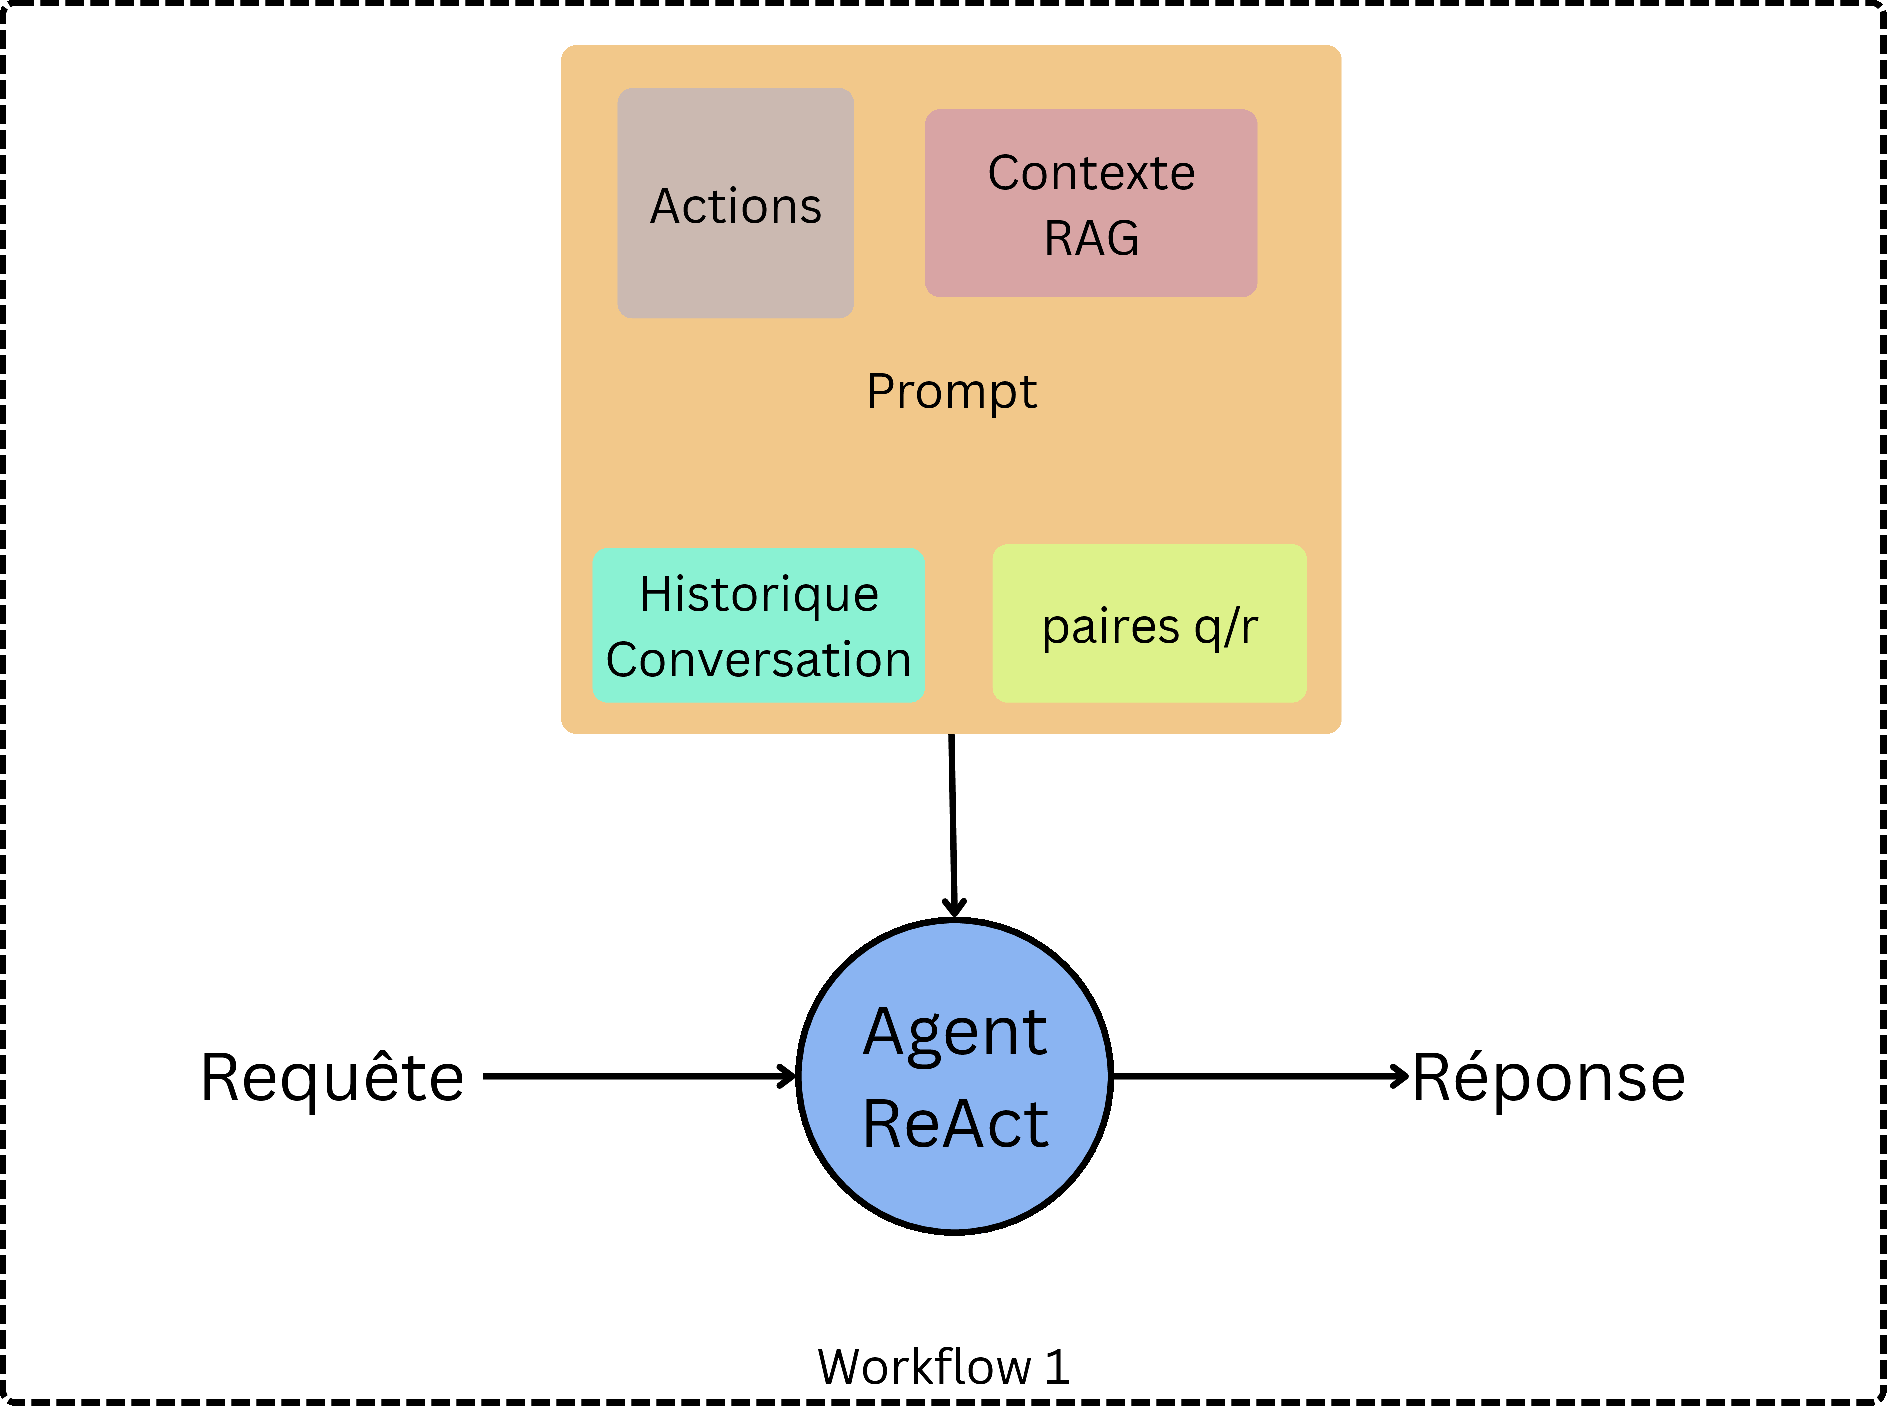
\includegraphics[keepaspectratio,height=8cm]
    {images/workflow_1.pdf}%
    \caption{Première conception agentique}%
\end{figure}
Cette première version, représentée par le Workflow 1, avait l’avantage de la simplicité et permettait de traiter correctement des cas d’utilisation de base. Cependant, cette centralisation montrait rapidement ses limites : l’agent produisait parfois des hallucinations, et surtout, les paires question/réponse, qui représentent des données strictes et validées, n’étaient pas toujours respectées à 100 \%. L’agent les traitait comme de simples éléments de contexte, alors qu’elles auraient dû être prioritaires par rapport au reste. Ce constat nous a conduit à réfléchir à une séparation des rôles pour mieux contrôler le processus de génération.

\subsection{Approche 2 – Agent double}
Dans la deuxième approche, nous avons introduit un Agent QR dédié à la gestion des paires question/réponse. Son rôle est de vérifier si ces paires sont suffisantes pour répondre à la requête. 
\begin{figure}[H]%
    \centering
    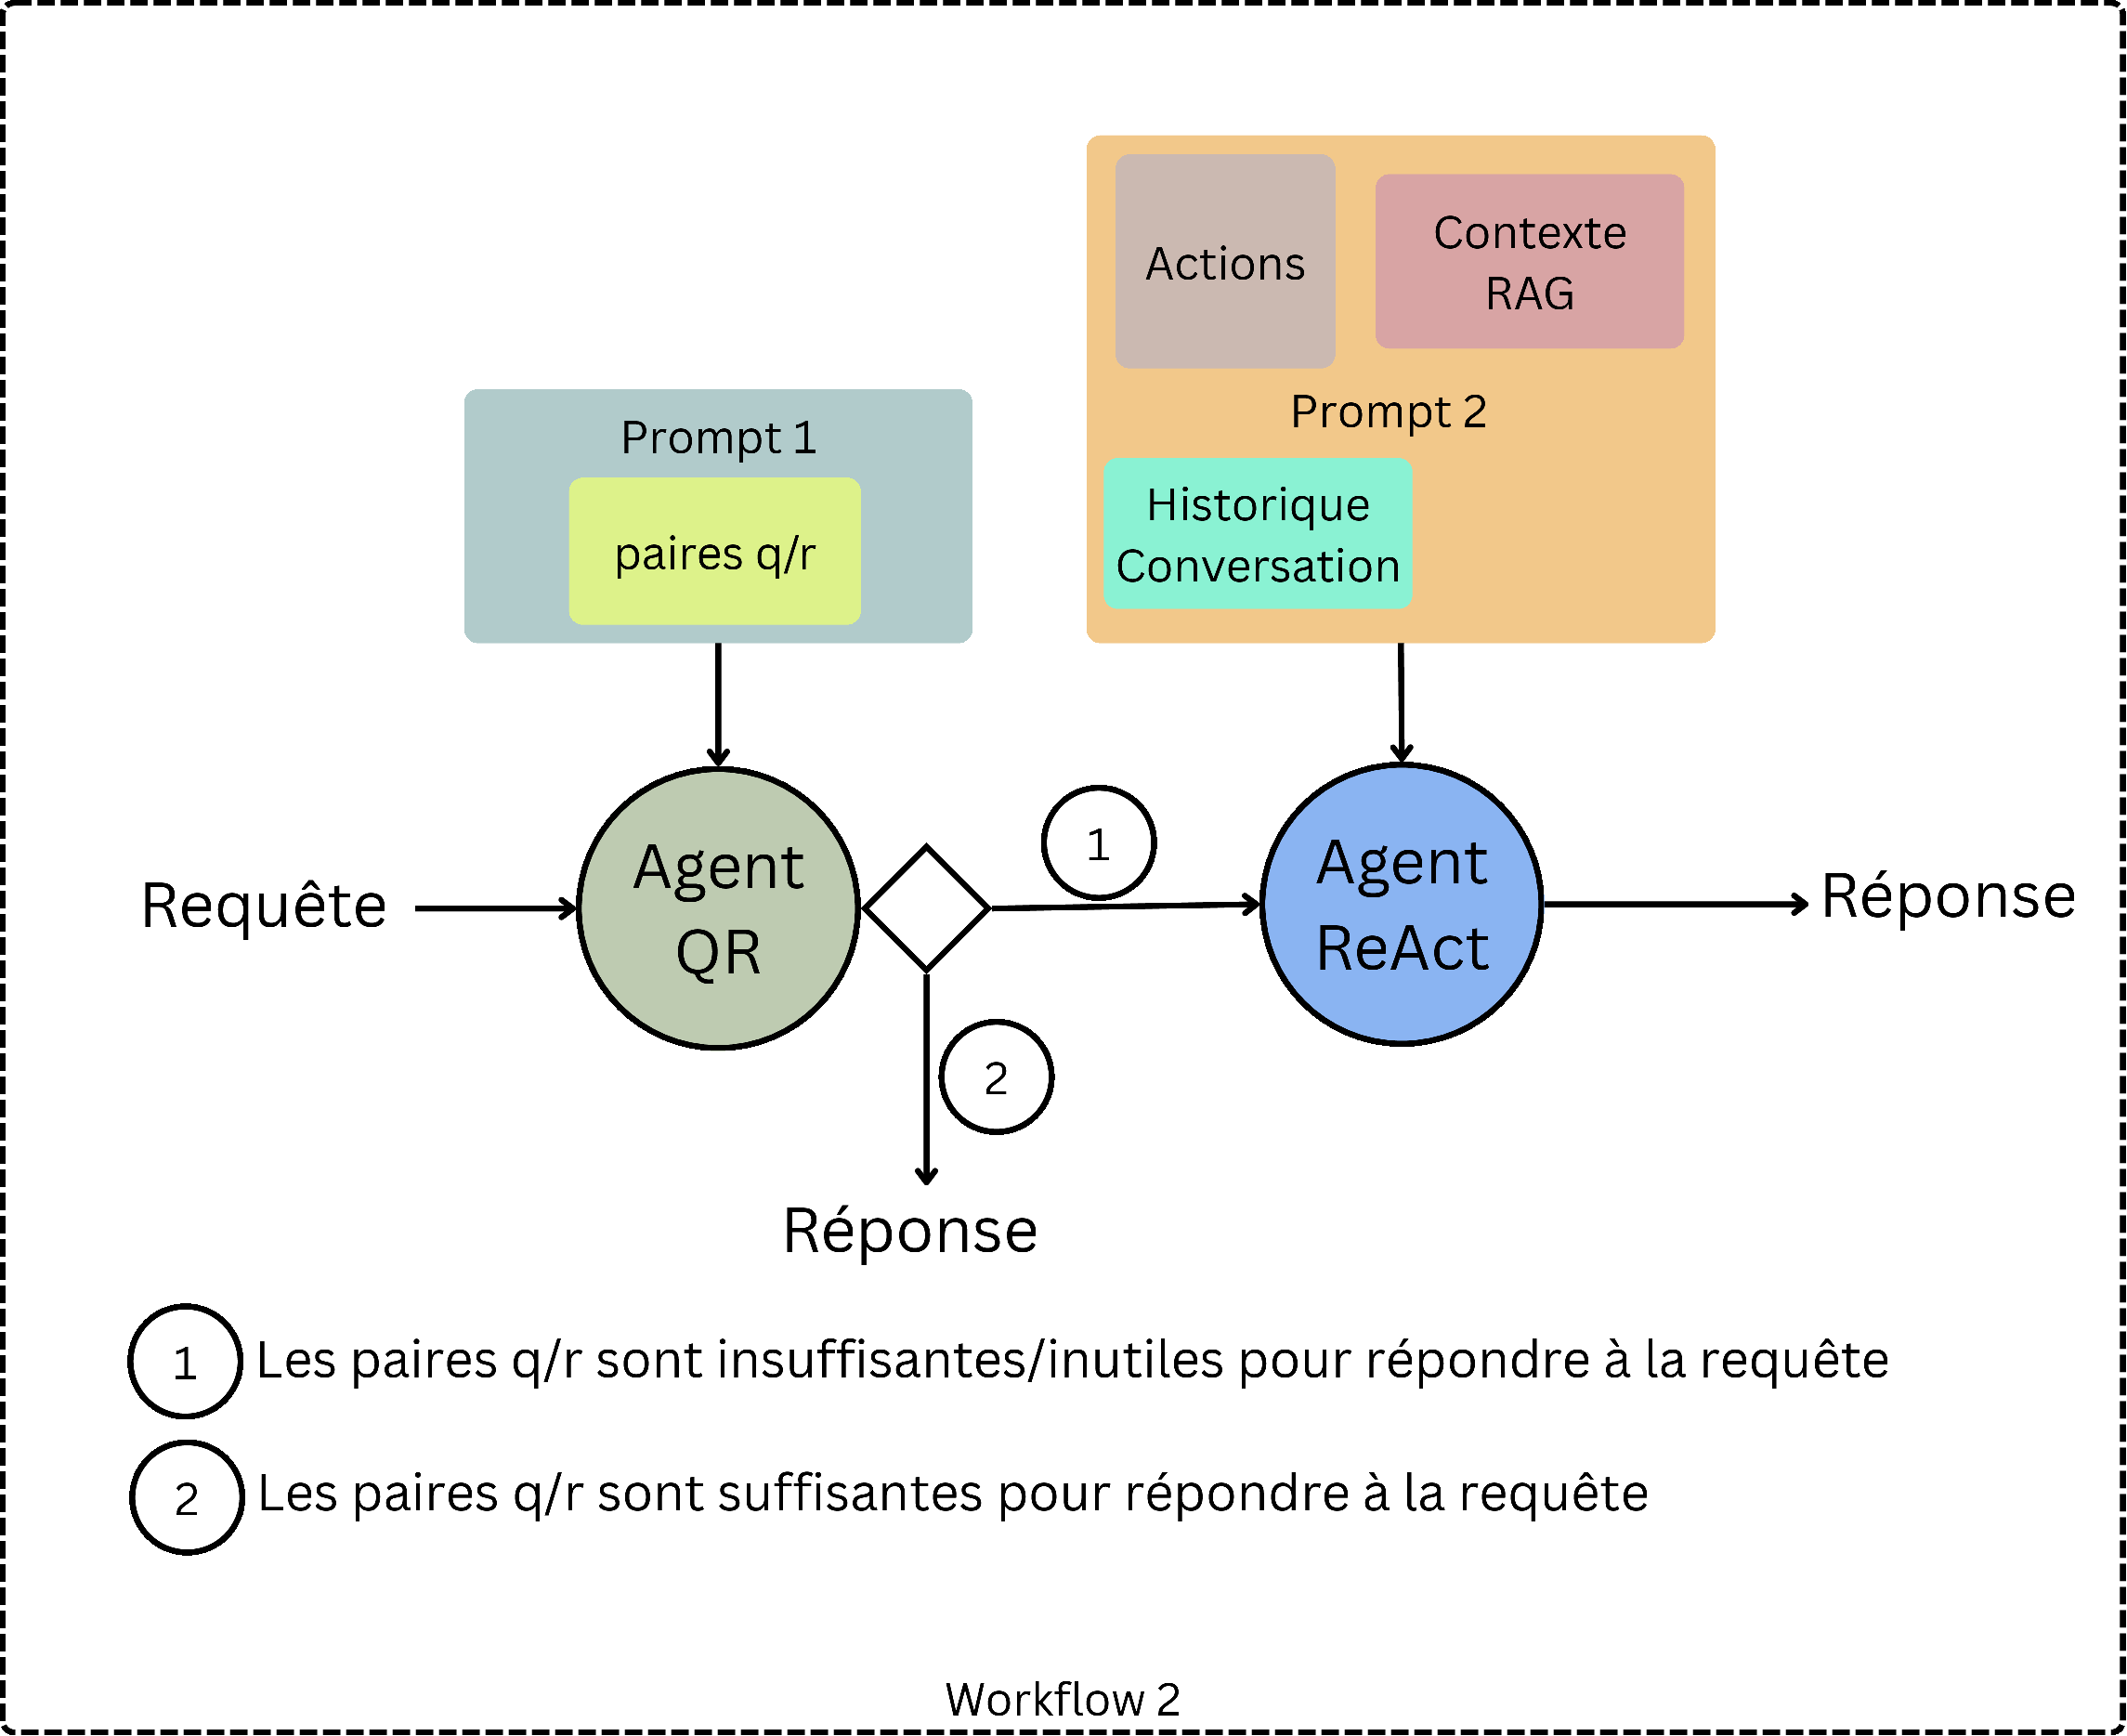
\includegraphics[keepaspectratio,height=8cm]
    {images/workflow_2.pdf}%
    \caption{Deuxième conception agentique}%
\end{figure}
Comme le montre la figure, deux cas sont alors possibles : si les paires sont jugées insuffisantes ou inutiles, une réponse directe peut être donnée par cet agent, ou bien la requête est transmise à l’agent ReAct avec éventuellement un extrait des paires jugées pertinentes. Si au contraire les paires Q/R suffisent, la réponse est produite directement. Ce mécanisme a permis de renforcer la priorité des Q/R et de mieux les exploiter. De plus, cette séparation a légèrement réduit la longueur du prompt, puisque tout le contexte n’était plus injecté dans un seul agent. Cependant, malgré cette amélioration, nous avons constaté que l’historique de conversation restait trop gourmand et prenait encore trop de place dans le prompt. D'où, l’agent continuait à diluer le contexte, perdait parfois des informations importantes et générait des réponses imprécises.
\subsection{Approche 3 – Multi-agents}
C’est pour résoudre ces problèmes que nous avons conçu une architecture plus avancée représentée par la troisième figure (Workflow 3).
\begin{figure}[H]%
    \centering
    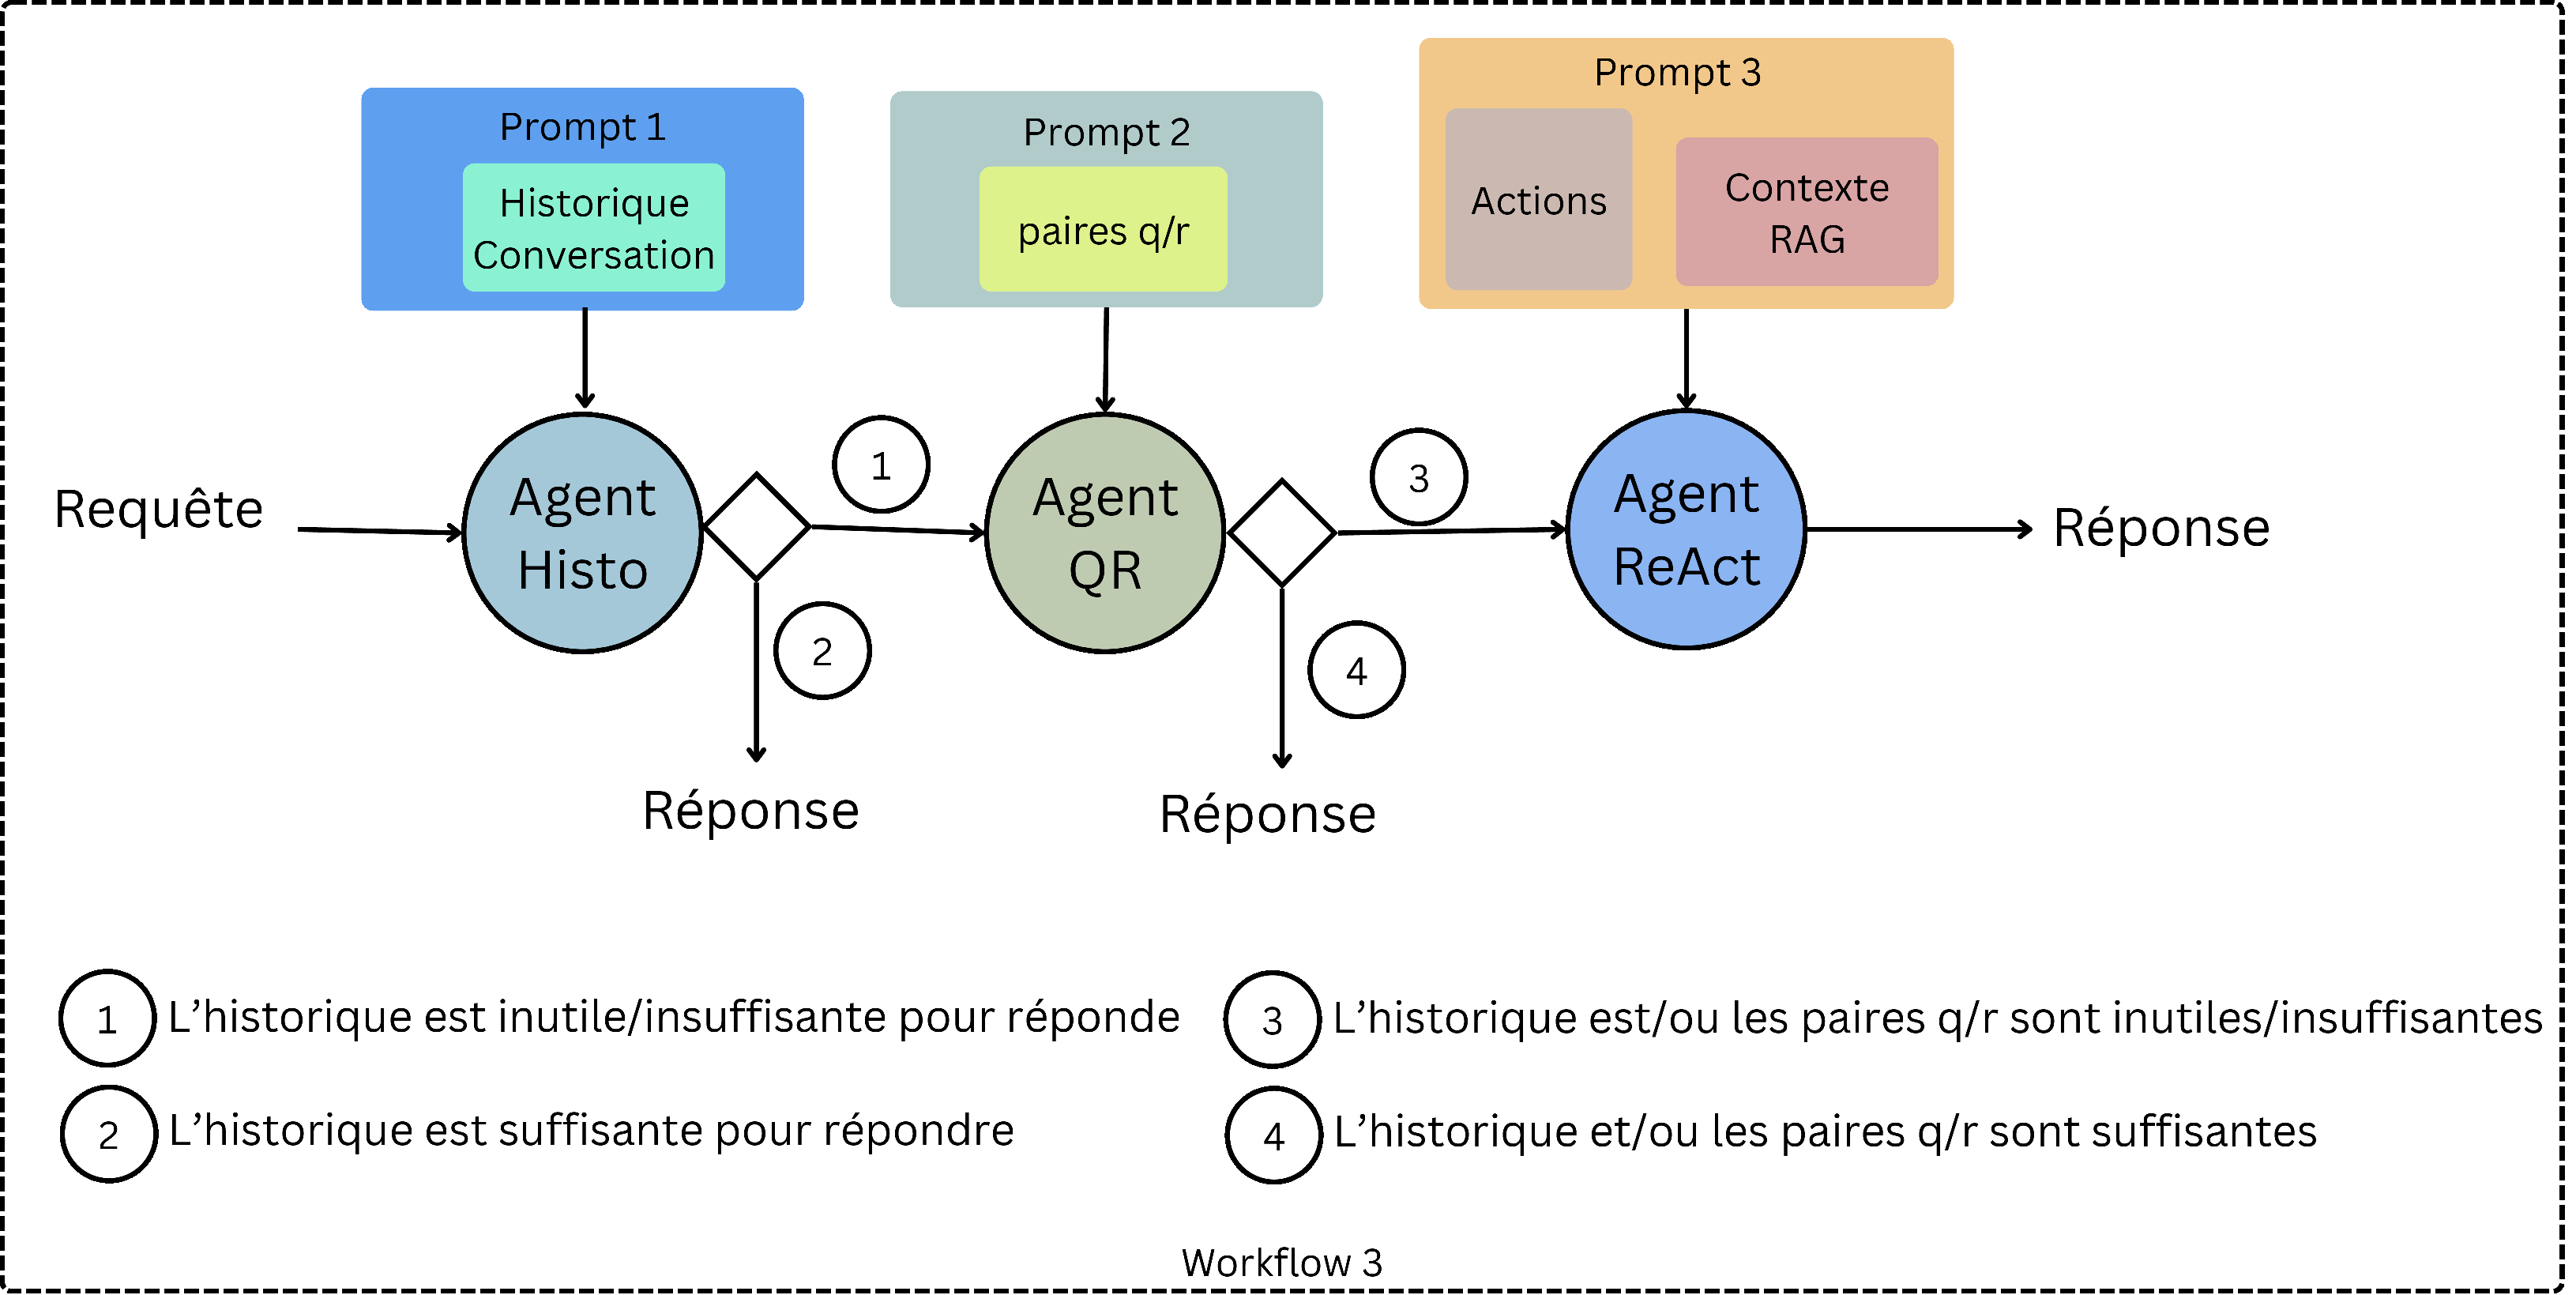
\includegraphics[keepaspectratio,height=8cm]
    {images/workflow_3.pdf}%
    \caption{Troisième conception agentique}%
\end{figure}
Ici, la requête passe d’abord par un Agent Histo, qui analyse la relation entre la question et l’historique de la conversation. L’idée est de vérifier si la réponse existe déjà dans les échanges passés, ou si un extrait de l’historique peut enrichir la compréhension. Si l’historique suffit, une réponse directe est produite, sinon la requête (éventuellement enrichie d’un extrait pertinent) est transmise à l’Agent QR, qui joue son rôle habituel de vérification des paires question/réponse. Là encore, deux cas se présentent : si les Q/R (seules ou combinées à l’historique) sont suffisantes, une réponse est générée, sinon la requête est finalement confiée à l’Agent ReAct. Ce dernier reçoit donc un prompt allégé et filtré, contenant uniquement les parties utiles de l’historique et des paires Q/R, ce qui lui permet de raisonner plus efficacement et de produire une réponse pertinente et cohérente.
\begin{figure}[H]%
    \centering
    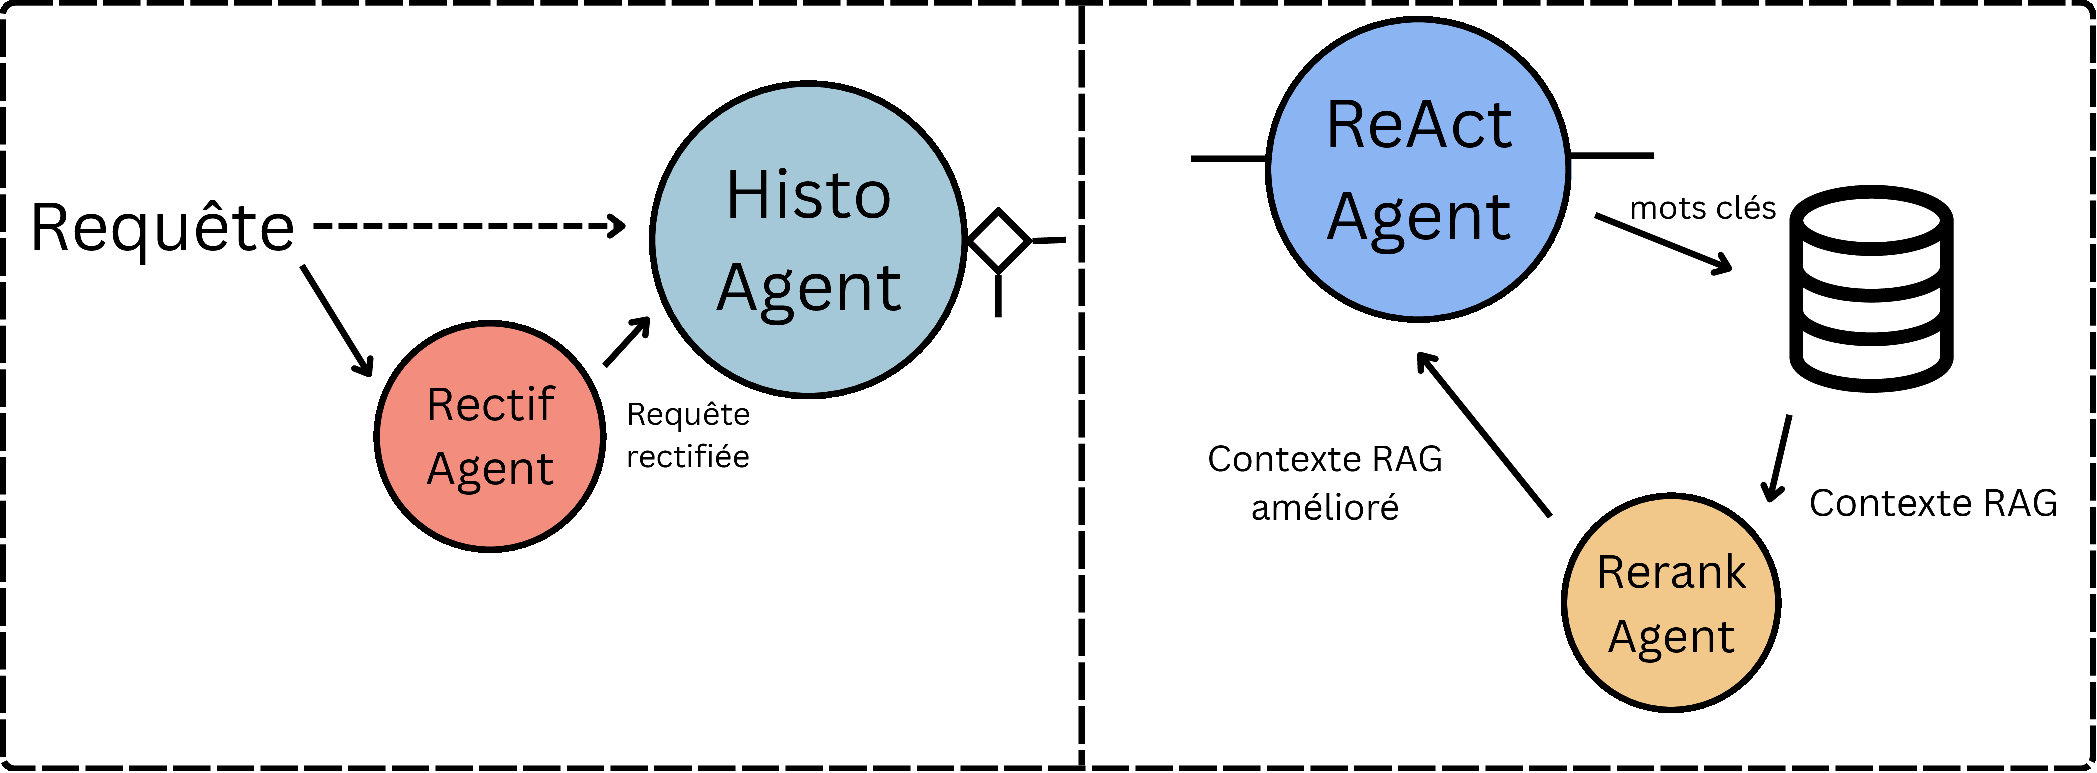
\includegraphics[keepaspectratio,width=\textwidth]
    {images/enhancements.pdf}%
    \caption{Améliorations dans l'architecture}%
    \label{fig:enhance}
\end{figure}
Pour renforcer encore la précision et l'efficacité de cette architecture, nous avons introduit des améliorations ciblées, comme illustré dans la figure \ref{fig:enhance}. Un agent de rectification (Rectif Agent) est intégré à l'Agent Histo pour raffiner la requête, corrigeant les ambiguïtés, les fautes de frappe et capturant mieux l'intention de l'utilisateur. Par ailleurs, un agent de reranking (Rerank Agent) optimise le contexte RAG récupéré en extrayant des mots clés pertinents, réorganisant les informations pour une pertinence accrue avant leur transmission à l'Agent ReAct. Ces ajouts minimisent les erreurs sémantiques et améliorent la qualité des réponses.

En conclusion, cette évolution progressive (du modèle centralisé vers une architecture multi-agents) nous a permis de réduire les hallucinations, de donner aux paires Q/R leur priorité stricte, et d’alléger les prompts pour améliorer la précision. Même en termes séquentiels, l’assistant a montré une performance remarquable, produisant des réponses plus justes, mieux contextualisées et adaptées à la requête de l’utilisateur.

\section{Choix des frameworks et modèles pour les agents}

La conception de notre plateforme repose sur des choix ciblés qui influencent directement l'architecture agentique et les capacités RAG, en alignant ces décisions sur l'objectif de créer une solution scalable et personnalisable pour la gestion de chatbots. Ces sélections, centrées sur les frameworks RAG et les modèles de langage, visent à optimiser la précision, la flexibilité et l'efficacité des flux conversationnels, tout en préparant une implémentation détaillée dans le chapitre dédié à la réalisation. 

\subsection{Comparaison des frameworks RAG}

La mise en œuvre d’une architecture agentique reposant sur des capacités avancées de RAG nécessite le recours à des frameworks spécialisés. Plusieurs solutions existent aujourd’hui, mais les deux plus largement adoptées dans la communauté sont LangChain et Llamaindex. Ces bibliothèques fournissent des abstractions de haut niveau pour le chaînage de LLMs, la gestion de contextes complexes, l’intégration de sources de données variées et la mise en place de pipelines de raisonnement multi-agents.

\subsubsection{LangChain}
LangChain \cite{langchain} est un framework principal utilisé pour l’orchestration des agents et le chaînage des composants dans les pipelines RAG. La figure \ref{fig:langchain_stack} illustre son écosystème et ses extensions, organisé en plusieurs couches.
\begin{figure}[H]%
\centering
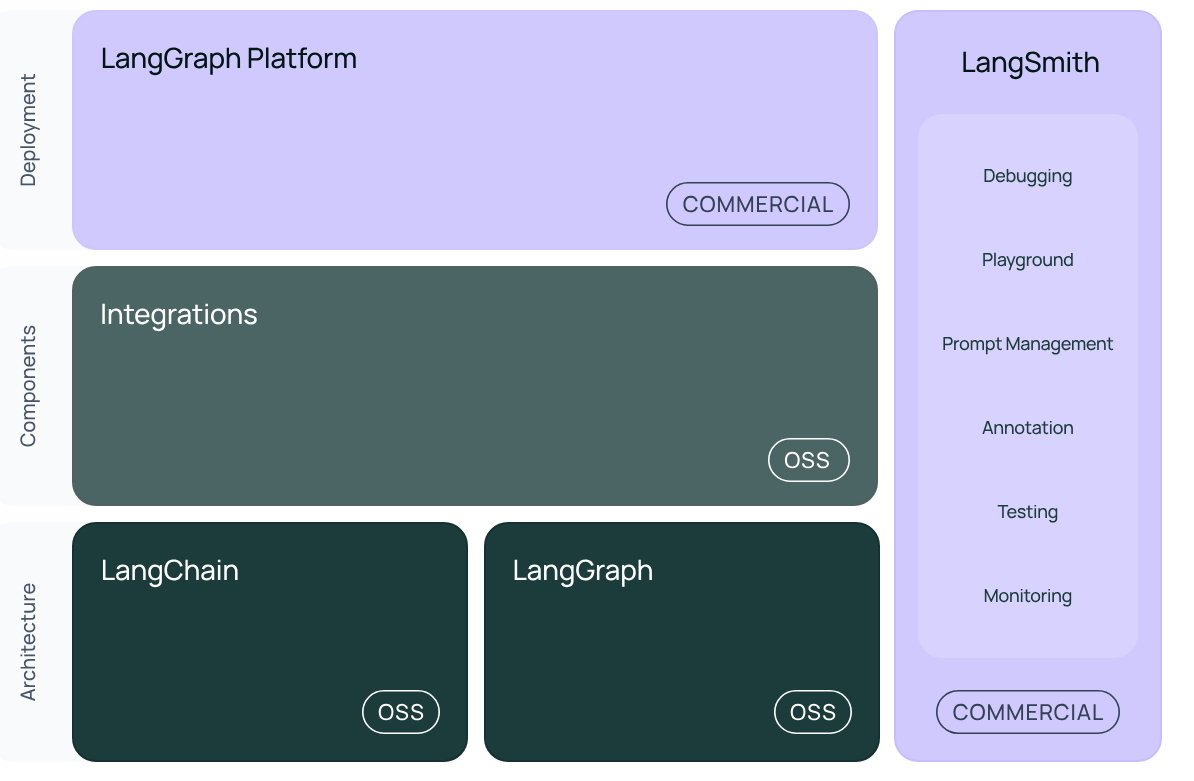
\includegraphics[keepaspectratio,height=8cm]
{images/langchain_stack.png}%
\caption{Écosystème et architecture de LangChain \cite{langchain_docs}}%
\label{fig:langchain_stack}
\end{figure}
L’architecture comprend LangChain et LangGraph, tous deux open source : LangChain fournit les briques de base pour l’orchestration séquentielle, tandis que LangGraph permet de modéliser des workflows complexes sous forme de graphes. La couche des composants (intégrations) open source assure la connexion avec des bases de données, des APIs et des outils externes, facilitant l’intégration de sources de données variées dans notre microservice RAG. Le déploiement est supporté par la LangGraph Platform, une solution commerciale offrant scalabilité et supervision dans un environnement managé. En outre, LangSmith, une suite d’outils commerciaux, couvre le cycle de vie des agents avec des fonctionnalités de debugging, gestion des prompts, annotation, tests et monitoring, renforçant la traçabilité. Le principal atout de LangChain réside dans sa vaste communauté, qui fournit une abondance de ressources et d’exemples, soutenant son adoption dans notre architecture.
\subsubsection{Llamaindex}
Llamaindex \cite{llamaindex} est un framework spécialisé dans la récupération et la gestion fine du contexte, conçu pour optimiser l’indexation et l’interrogation de bases de connaissances complexes. Parmi ses points forts, LlamaHub se distingue par ses capacités d’intégration, permettant de connecter une vaste gamme de sources de données hétérogènes telles que des fichiers et des bases de données externes, grâce à une évolution rapide et une compatibilité croissante avec divers connecteurs.
\begin{figure}[H]%
\centering
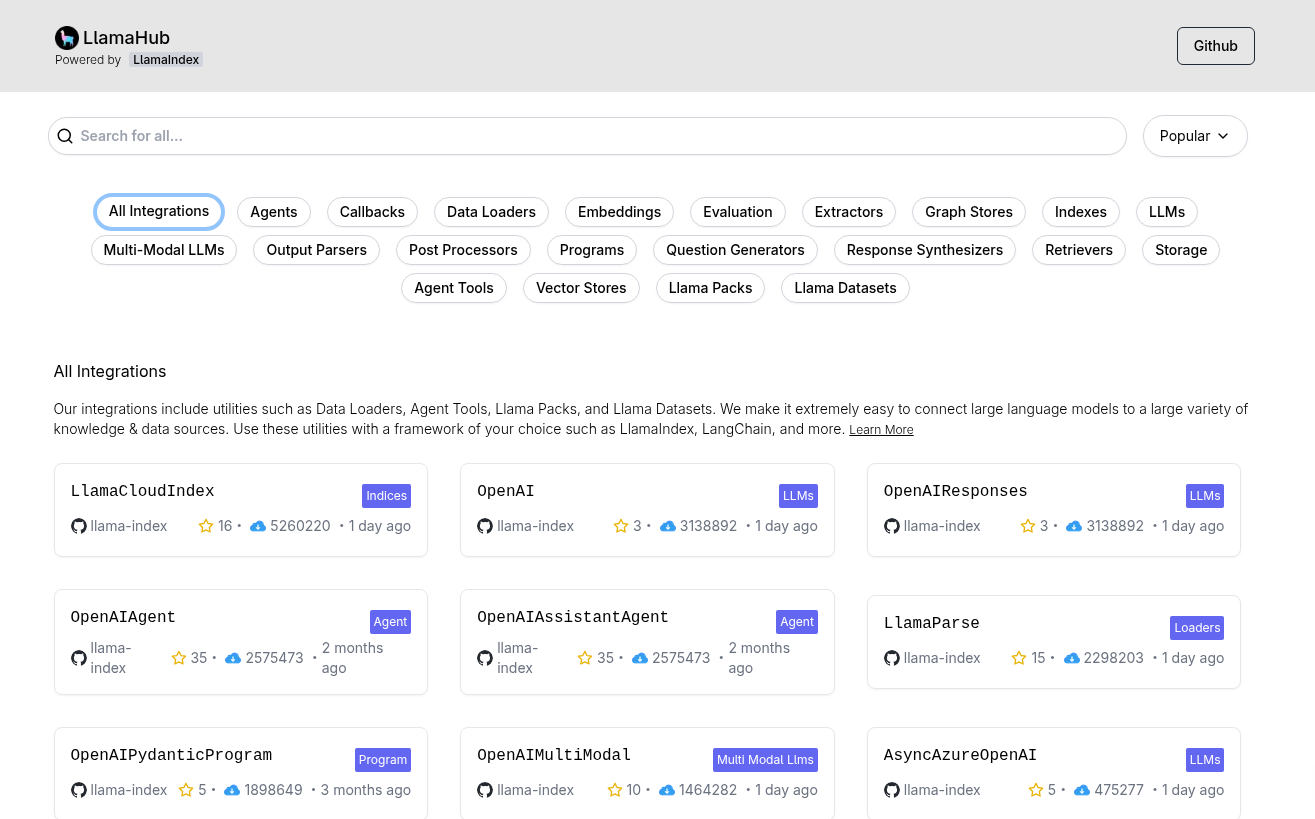
\includegraphics[keepaspectratio,height=7cm]
{images/llamahub.png}%
\caption{Librairie des intégrations de Llamahub}%
\label{fig:llamahub}
\end{figure}
De plus, LlamaCloud, une plateforme commerciale de Llamaindex, offre des fonctionnalités avancées pour le parsing (chargement) de données, l’ingestion, la récupération, l’extraction de données structurées et bien plus encore. Elle propose LlamaParse, un outil révolutionnaire qui automatise le traitement des documents avec une précision remarquable, renforçant les capacités de récupération sémantique. Ces atouts font de Llamaindex une option puissante pour des scénarios nécessitant une pertinence très élevée, bien que ses fonctionnalités avancées soient payantes, ce qui a limité son adoption complète dans notre projet.

Ce framework était testé en parallèle afin d’évaluer ses capacités spécifiques en récupération et en gestion fine du contexte.  

\subsubsection{Résultats expérimentaux}
Afin d’évaluer leurs performances respectives dans notre solution, nous avons conçu deux prototypes distincts, l’un basé sur LangChain et l’autre sur Llamaindex, dans deux scenarios différents, le premier avec des fichiers simples de taille réduite, le deuxième avec un fichier complexe de plus grande taille. en veillant à garder une configuration identique dans deux environnements similaires et isolés:
\begin{itemize}[label=\textbullet]
    \item Modèle d’embedding : text-embedding-3-small
    \item LLM utilisé : gpt-4o-mini
    \item Vector store : PgVector (deux conteneurs distincts pour séparer la persistance et la recherche)
    \item Données de test : trois fichiers hétérogènes mais simples (TXT, PDF, CSV) [scénario 1], un fichier PDF complexe [scénario 2]
    \item Paramètres de découpage : taille de chunk = 500, chevauchement = 50
\end{itemize}

L’évaluation a porté sur plusieurs aspects : temps de parsing, découpage, génération des embeddings, consommation de tokens, pertinence du rappel (retrieval) et documentation.

\begin{table}[H]
\centering
\caption{Performances de parsing et d’embedding (scénario 1)}
\begin{tabular}{|l|c|c|}
\hline
\textbf{Mesures} & \textbf{LangChain} & \textbf{Llamaindex} \\
\hline
Temps de parsing (s) & 0.3 & 0.3 \\
Temps de découpage (s) & 0.02 & 0.05 \\
Temps d’embedding (s) & 0.04 & 0.25 \\
Consommation de tokens (embedding) & stricte & légèrement plus élevée \\
\hline
\end{tabular}
\end{table}

\begin{table}[H]
\caption{Performances globales (scénario 2)}
\centering\resizebox{\linewidth}{!}{
    \begin{tabular}{|l|c|c|}
    \hline
    \textbf{Mesures} & \textbf{LangChain} & \textbf{Llamaindex} \\
    \hline
    Temps de parsing (s) & 0.3 & 1.11 \\
    Temps de découpage (s) & 5.56 & 9.48 \\
    Temps d’embedding (s) & 1.45 & 1.54 \\
    Consommation de tokens (embedding) & stricte & légèrement plus élevée \\
    Rappel (retrieval) & 2/3 des données pertinentes & 3/4 des données pertinentes \\
    Consommation de tokens (prompting) & raisonnable & plus élevée \\
    \hline
    \end{tabular}
}
\end{table}

\begin{table}[H]
\caption{Complexité et documentation}
\centering\resizebox{\linewidth}{!}{
\begin{tabular}{|l|c|c|}
\hline
\textbf{Aspect} & \textbf{LangChain} & \textbf{Llamaindex} \\
\hline
Complexité de la documentation & Plus facile de trouver du code & Documentation plus claire \\
Organisation des packages & En cours de réorganisation & Bien séparés \\
\hline
\end{tabular}}
\end{table}

\subsubsection{Analyse et choix}
Les résultats montrent que LangChain est généralement plus performant en parsing et en découpage, avec une consommation de tokens plus stricte. En revanche, Llamaindex obtient de meilleurs résultats en termes de pertinence du rappel (3/4 des données retrouvées contre 2/3 pour LangChain), au prix d’une consommation plus importante en temps et en tokens.

D’un point de vue développement, LangChain dispose d’une plus grande quantité de ressources communautaires et d’exemples de code facilement accessibles, tandis que Llamaindex propose une meilleure documentation structurée et une séparation plus claire des modules.

Compte tenu de ces observations, notre choix s’est porté sur LangChain pour l’orchestration principale, en raison de sa performance et de sa flexibilité, tout en gardant la possibilité d’intégrer certains composants de Llamaindex dans des cas spécifiques où la pertinence du contexte est prioritaire.  

\subsection{Choix agentiques}
Bien que les frameworks RAG, tels que LangChain et Llamaindex, supportent la réalisation de flux agentiques, nous cherchons à exploiter plus d'élasticité pour répondre aux besoins spécifiques de notre plateforme. Cette ambition nous a conduit à explorer des solutions plus avancées pour l’orchestration.
\subsubsection{LangGraph}
LangGraph \cite{langgraph}, une extension puissante de LangChain, repousse les limites de l’orchestration en modélisant les chaînes et agents sous forme de graphes dynamiques. Cette approche permet de gérer des workflows complexes avec suivi d’état, retours en arrière, branches et boucles, répondant aux exigences de notre architecture multi-agents.

Construit sur les bases de LangChain, LangGraph offre une personnalisation avancée, idéale pour coordonner les agents au sein du microservice Orchestrateur.
Le tableau \ref{table:chainVSgraph} compare LangChain et LangGraph, soulignant leur complémentarité dans notre solution.

\subsubsection{Analyse et choix}
\begin{table}[H]
\caption{Comparaison entre LangChain et LangGraph}
\centering\resizebox{\linewidth}{!}{
\begin{tabular}{|p{0.2\linewidth}|p{0.4\linewidth}|p{0.4\linewidth}|}
\hline
\textbf{} & \textbf{LangChain} & \textbf{LangGraph} \\
\hline
\textbf{Utilisation principale} & Construction et chaînage linéaire des tâches LLM & Gestion de workflows complexes, avec état, multi-agents. \\
\hline
\textbf{Structure} & Séquentielle et modulaire (les tâches sont exécutées dans un ordre spécifique). & Basée sur des graphes : permet d'aller et venir entre les états, avec branchements et boucles. \\
\hline
\textbf{Support des agents} & Agents linéaires (chemin unique). & Agents multi-agents personnalisés. \\
\hline
\end{tabular}}
\label{table:chainVSgraph}
\end{table}

LangGraph a facilité l’évolution de notre architecture agentique, permettant une transition fluide entre les approches (agent unique à multi-agents) grâce à sa flexibilité. Sa capacité à intégrer et personnaliser des agents, comme l’Agent Histo ou l’Agent QR, a optimisé la coordination et réduit les hallucinations, renforçant l’adaptabilité de la plateforme en alignement avec l’objectif de personnalisation.

\subsection{Choix des modèles de langage (LLMs)}
Un choix important a concerné la sélection des modèles de langage utilisés pour le raisonnement et la génération de réponses. Plusieurs modèles d’OpenAI ont été testés : GPT-4o-mini, GPT-4o, o3-mini, GPT-4.1-nano, GPT-5-mini et GPT-5-nano.  

Les modèles de petite taille, comme 4o-mini ou 5-nano ou 4.1-nano, présentent l’avantage d’un coût très faible et d’une consommation réduite en tokens. Cependant, ils produisent souvent des réponses plus courtes et résumées, en raison d’un biais lié à leur taille limitée. À l’inverse, les modèles plus puissants tels que GPT-4o ou o3-mini offrent une meilleure précision et une compréhension contextuelle plus riche, mais ils nécessitent davantage de temps de traitement et un coût plus élevé. Les modèles intermédiaires, comme 4o-mini et 5-mini, constituent un compromis intéressant, bien que les anciens modèles comme o3-mini et GPT-4o soient plus coûteux que leurs équivalents récents.  

\begin{table}[H]
\centering
\caption{Comparaison synthétique des modèles de langage testés (prix par 1M tokens) \cite{openai-pricing}}
\resizebox{\textwidth}{!}{%
\begin{tabular}{|l|c|c|c|c|}
\hline
Modèle & Input & Cached Input & Output & Points faibles \\
\hline
GPT-5-mini & \$0.25 & \$0.025 & \$2.00 & Plus lent que nano, coût moyen \\
GPT-5-nano & \$0.05 & \$0.005 & \$0.40 & Réponses courtes, biais vers le résumé \\
GPT-4.1-mini & \$0.40 & \$0.10 & \$1.60 & Conso. tokens plus élevée, coût moyen \\
GPT-4.1-nano & \$0.10 & \$0.025 & \$0.40 & Couverture contextuelle limitée \\
GPT-4o-mini & \$0.15 & \$0.075 & \$0.60 & Réponses plus simples, moins détaillées \\
o3-mini & \$1.10 & \$0.55 & \$4.40 & Ancien modèle, tokens gourmands \\
\hline
\end{tabular}
}
\end{table}

Cette hiérarchisation a permis de définir une stratégie équilibrée : recourir à des modèles légers pour les requêtes rapides et peu critiques, et réserver les modèles plus grands aux tâches sensibles nécessitant un haut niveau de fiabilité.
Par conséquent, GPT-5-mini est employé dans le splitting agentique et le reranking agentique, où sa rapidité et son efficacité en tokens permettent de décomposer et prioriser les éléments contextuels longs avec précision.\\
Pour les tâches de contexte moins long, comme l’analyse d’historiques dans l’Agent Histo ou l’évaluation des paires question/réponse dans l’Agent QR ou la rectification, GPT-4.1-nano, GPT-4o-mini, GPT-5-nano sont privilégiés, offrant une couverture contextuelle adéquate à un coût raisonnable. GPT-5-mini est réservé à l’Agent ReAct pour le raisonnement final, garantissant une précision optimale lors de la génération de réponses.

\section{Conclusion}
Ce chapitre a permis de mettre en évidence les choix architecturaux et technologiques fondamentaux de notre solution. L’approche microservices, combinée à l’utilisation des services managés d’Azure et des frameworks RAG, assure à la fois scalabilité, maintenabilité et performance. L’évolution progressive vers une architecture multi-agents a renforcé la fiabilité des réponses et réduit les hallucinations. Enfin, la comparaison des modèles et frameworks confirme que nos sélections technologiques constituent un compromis optimal entre coût, performance et pertinence. Découvrons dans le chapitre suivant comment l'implémentation est effectuée.
